\documentclass{template/openetcs_article}
% Use the option "nocc" if the document is not licensed under Creative Commons
%\documentclass[nocc]{template/openetcs_article} 
\usepackage{rotating,url,color}
\graphicspath{{./template/}{.}{./images/}}
\usepackage{graphicx}
%\usepackage{draftwatermark}
%\SetWatermarkLightness{0.85}
%\SetWatermarkAngle{25}
%\SetWatermarkScale{2}
%\SetWatermarkFontSize{2cm}
%\SetWatermarkText{Intermediate}

% Addded to manage two-lined url @MatthieuPERIN
\usepackage{hyperref}
% option to have non visible box on links
\hypersetup{hidelinks}

\newcommand{\sysmlicon}[1]{\includegraphics{icons/#1}}

\begin{document}
\frontmatter
\project{openETCS}


%Please do not change anything above this line
%============================
% The document metadata is defined below


%assign a report number here
\reportnum{OETCS/WP2/D2.4~--~00.04}

%define your workpackage here
\wp{Work-Package 2: ``Definition''}

%set a title here
\title{OpenETCS methods}

%set a subtitle here
\subtitle{ Definition of the methods used to perform the formal description}

%set the date of the report here
\date{September 2013}

%define a list of authors and their affiliation here

\author{Marielle Petit-Doche}
\affiliation{Systerel}


\author{David Mentré}
\affiliation{Mitsubishi Electric R\&D Centre Europe}

\author{Mathias Güdemann}
\affiliation{Systerel}


% define the coverart
\coverart[width=350pt]{openETCS_EUPL}
 
%define the type of report
\reporttype{Definition}


\begin{abstract}
This document give first an introduction to formal  methods.
In a second part, it proposes the method to  fllow during the openETCs project according to the methodology selection.

\end{abstract}

%=============================
%Do not change the next three lines
\maketitle
\tableofcontents
\listoffiguresandtables
\newpage
%=============================

\begin{tabular}{|p{4.4cm}|p{8.7cm}|}
\hline
\multicolumn{2}{|c|}{Document information} \\
\hline
Work Package &  WP2  \\
Deliverable ID or doc. ref. & D2.4\\
\hline
Document title & Definition of the methods used to perform the formal description \\
Document version & 00.04 \\
Document authors (org.)  & Marielle Petit-Doche (Systerel)  \\
  & David Mentré (Mitsubishi Electric R\&D Centre Europe)  \\
  & Mathias Güdemann (Systerel)  \\
\hline
\end{tabular}

\begin{tabular}{|p{4.4cm}|p{8.7cm}|}
\hline
\multicolumn{2}{|c|}{Review information} \\
\hline
Last version reviewed & 00.01 \\
\hline
Main reviewers & S. Baro (SNCF) \\
& P. Mahlmann (DB), B. Hekele (DB)\\
& H. Hungar (DLR), M. Behrens (DLR) \\
& J. Welte ( TU-BS) \\
\hline
\end{tabular}

\begin{tabular}{|p{2.2cm}|p{4cm}|p{4cm}|p{2cm}|}
\hline
\multicolumn{4}{|c|}{Approbation} \\
\hline
  &  Name & Role & Date   \\
\hline  
Written by    &  Marielle Petit-Doche & T2.4 Sub-Task Leader  & September 2013 \\
& David Mentré & & \\
& Matthias Güdemann & & \\
\hline
Approved by & Gilles Dalmas & WP2 leader & \\
\hline
\end{tabular}

\begin{tabular}{|p{2.2cm}|p{2cm}|p{3cm}|p{5cm}|}
\hline
\multicolumn{4}{|c|}{Document evolution} \\
\hline
Version &  Date & Author(s) & Justification  \\
\hline  
00.01 & 03/05/2013 & M. Petit-Doche &  Incorporation of section on formal methods written by David Mentré \\
\hline  
00.02 & 2013-05-16 & D. Mentré &  Incorporation of formal reviews in
the document \\
\hline  
00.03 & 03/05/2013 & M. Petit-Doche &  Remaining remarks of formal reviews \\
\hline  
00.04 & 26/09/2013 & M. Petit-Doche, D. Mentré & First version of sections 7, 8 and 9   \\
\hline  

\end{tabular}



% The actual document starts below this line
%=============================

%%%%%%%%%%%%%%%%%%%%%%%%%%%%%%%%%%%%%%%%%%%%%%%%%%%%%%%%%%%%%%
%%%              My macros (=> Sylvain Baro)               %%%
%%%%%%%%%%%%%%%%%%%%%%%%%%%%%%%%%%%%%%%%%%%%%%%%%%%%%%%%%%%%%%
\newcommand{\tbd}{\colorbox{cyan}{\%\%To Be Defined\%\%}}
\newcommand{\tbc}{\colorbox{cyan}{\%\%To Be Confirmed\%\%}}
\newcommand{\todo}[1]{\colorbox{cyan}{\%\%{#1}\%\%}}
\newlength{\origindent}

\newenvironment{issue}{
	\begin{quote}
	\begin{itshape}Open Issue. 
}{
	\end{itshape}
	\end{quote}
}

\newenvironment{comment}{
	\begin{quote}
	\begin{itshape}Comment. 
}{
	\end{itshape}
	\end{quote}
}

\newenvironment{justif}{
	\begin{quote}
	\begin{itshape}Justification. 
}{
	\end{itshape}
	\end{quote}
}
%% Requirements.


\newcounter{reqnum}
\setcounter{reqnum}{0}
\newcounter{subreqnum}
\newcounter{subsubreqnum}
\newlength{\partopbuf}
\newlength{\topbuf}

% Automated numbering versions of the macros
\newcommand{\req}[1]{\addtocounter{reqnum}{1} \setcounter{subreqnum}{0}
	\begin{description}\item[{\small\reqt-X-\thereqnum}] #1\end{description}
}

\newcommand{\subreq}[1]{
	\addtocounter{subreqnum}{1} \setcounter{subsubreqnum}{0}
	\addtolength{\leftmargini}{1cm}
	\begin{description}
	\item[\hspace{0.5cm}{\small\reqt-X-\thereqnum.\thesubreqnum}] #1
	\end{description}
	\addtolength{\leftmargini}{-1cm}
}

\newcommand{\subsubreq}[1]{
	\addtocounter{subsubreqnum}{1}
	\addtolength{\leftmargini}{2cm}
	\begin{description}
	\item[\hspace{1cm}{\small\reqt-X-\thereqnum.\thesubreqnum.\thesubsubreqnum}] #1
	\end{description}
	\addtolength{\leftmargini}{-2cm}
}

% Fixed version of the commands
\newcommand{\reqfixed}[3]{\addtocounter{reqnum}{1} \setcounter{subreqnum}{0}
	\begin{description}\item[{\small\reqt-#1-#2}] #3\end{description}
}

\newcommand{\subreqfixed}[4]{
	\addtocounter{subreqnum}{1} \setcounter{subsubreqnum}{0}
	\addtolength{\leftmargini}{1cm}
	\begin{description}
	\item[\hspace{0.5cm}{\small\reqt-#1-#2.#3}] #4
	\end{description}
	\addtolength{\leftmargini}{-1cm}	
}

\newcommand{\subsubreqfixed}[5]{
	\addtocounter{subsubreqnum}{1}
	\addtolength{\leftmargini}{2cm}
	\begin{description}
	\item[\hspace{1cm}{\small\reqt-#1-#2.#3.#4}] #5
	\end{description}
	\addtolength{\leftmargini}{-2cm}	
}

% Citation of the requirement

% Citation of the reference (for markup purpose)
%\newcommand{\refreq}[1]{\textbf{#1}}

% Citation of the reference and text (for markup purpose)
% The purpose of this is to automatically replace the placeholder by the 
% full text. \fullrefreq{R-xxx}{} or \fullrefreq{R-xxx}{blabla} 
% will be replaced by \fullrefreq{R-xxx}{text of the R-xxx requirement} 
%\newcommand{\fullrefreq}[2]{\textbf{#1}: \textrm{#2}}


\def\reqt{R-WP2/D2.3.0}
% Start here

%%%%%%%%%%%%%%%%%%%%%%%%%%%%%%%%%%%%%%%%%%%%%%%%%%%%%%%%%%%%%%%


\section{Introduction}

The purpose of this document is to describe the specification and design activities for the OpenETCS project. The activities for safety, verification and validation are not in the scope of this document and will be described in WP4's documents.

To deal with a safety process, the specification and design activities shall follow the requirements of EN 50126, EN 50128 and EN 50129 and reflect usual activities for the development of railway critical systems (see D2.1  and D2.2).
This description is linked to the set of requirements defined for the OpenETCS project in D2.6.

\subsection{Motivation}

This document describes the process to  be applied  during the OpenETCS project to achieve the main goals of the OpenETCS project:

\paragraph{A semi-formal reference specification for the ETCS requirements and architecture, completed by strictly formal  models of sub-parts}
The first goal of the project is to propose a semi-formal specification of the ETCS on-board functionalities according to  UNISIG SUBSET-026, baseline 3.

The purpose of this model is:
\begin{itemize}
\item to enhance the understanding of the subset;
\item to be able to animate the model for testing and analysing purpose at system level;
\item to provide information on the completeness and soundness of the SUBSET-026;
\item to be used as a reference semi-formal specification for the implementation of an on-board unit
(by the OpenETCS project team and by industrial actors);
\end{itemize}

The output is a model, at least semi-formal, understandable by many formal approaches (SCADE,
Simulink, B tools, OpenETCS tool chain…) that can be given to all railway actors, and
if possible associated to SRS documents in the ERA database.

Thus, strictly formal models can be designed from this semi-formal model which allows for formal proofs of sub-parts of SUBSET-026. This will allow improving the understanding of the system, and will provide elements for verification and validation using formal proof.

The final goal is that industrial actors work with this model instead of the
natural language specification.
The objective is to cover as much as possible of the  functionality of the on-board unit described in SUBSET-026 and to show the capabilities of analyses of a complex system using formal approaches.

\paragraph{Definition the safety case concept for the full model and apply it on a subset of the on-board unit}
The safety strategy and the safety case concept required for the full validation of the product, compliant to the CENELEC standards shall be taken into account in all steps of the specification and design process. This will allow industrial actors to reuse the models and processes to develop certifiable products.

In particular the definition of the process shall take into account specification as well as verification and validation of the safety properties on the models. The outputs of WP4 (safety plan, safety case concept, verification plan and validation plan) will complete the description of the safety process.


\paragraph{Providing a tool chain and process/methodologies for developing
an on-board software that can fulfil the CENELEC requirements for SIL4 software}

The design process of the system and the associated tools of the tool chain shall be suitable to provide a certifiable product. For this purpose all steps of the process and the choice of the methods and tools shall be justified to ensure a safe approach to build an ETCS system.

The full safety process required to make OpenETCS \emph{certifiable} according to CENELEC 50126, 50128 and 50129 shall be described in detail. The safety process will detail precisely which activities are required, why they are required, and the choices that are made to claim that a safe design process is guaranteed.

The use of formal methods, supported by tools, is highly recommended in this safety process for specification, design, verification and validation of the certifiable product.

The tool chain should include model editors, code generators, verification tools (including formal provers), validation tools (including test generators, simulators,..), document generation, version management, maintenance facilities, \dots

\paragraph{Provide an executable software package generated from the specification of on-board ETCS}

An executable software of the specification shall be provided, as well as a non vital implementation of the on-board unit for laboratory test, simulation and as reference.

The output is the result of a functional implementation for the ETCS requirements and architecture which can be used by the industrial as reference. It will be a non-vital  implementation, able to be executed in real-time and in interaction with other components.


\subsection{Contents of this Document}

As the Quality Plan D1.3 focuses on means to apply during the OpenETCS project (for example open source approaches or Scrum organization) the aim of this document is to define the main steps which are necessary within the OpenETCS project to produce a certifiable system according to the CENELEC standards.
Safety, verification and validation activities are described in the outputs of WP4.

\todo{Give the references of WP4 deliverables}

The first part of this document focuses on the description of the mandatory steps of a life-cycle to design a critical system according to the CENELEC standards, as described in figure~\ref{fig:OETCSProcess}.

\begin{figure}[h]
  \centering
  \fbox{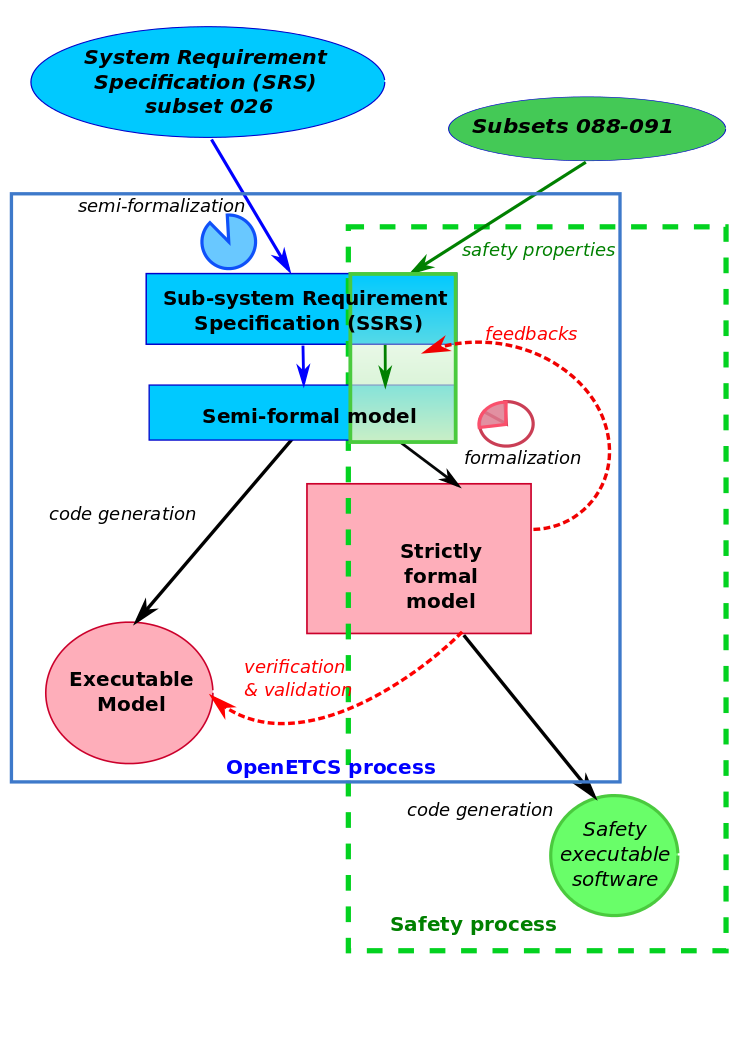
\includegraphics[width=4in]{OETCSProcess.png}}
  \caption{OpenETCS process}
  \label{fig:OETCSProcess}
\end{figure}


The proposed process for the OpenETCS project shall describe:
\begin{itemize}
\item how to design a semi-formal model of the on-board unit system from the SRS SUBSET-026 ;
\item how to design some subsets of the SRS SUBSET-026 within a safety process;
\item how to produce a running model of the application software of the on-board unit.
\end{itemize}

For the 2 first objectives, the semi-formal  model  shall take into account the safety constraints to apply to the design of a critical railway system.

The second part of this document describes the system to design during the OpenETCS project, as well as the scope of the safety activities on this system.

%%%%%%%%%%%%%%%%%%%%%%%%%%%%%%%%%%%%%%%%%%%%%%%%%%%%%%%%%%%%%%%

\section{Reference Documents}
\begin{itemize}
\item CENELEC EN 50126-1 --- 01/2000 --- \emph{Railways applications –- The specification and
demonstration of Reliability, Availability, Maintainability and Safety (RAMS) –- Part 1:
Basic requirements and generic process}
\item CENELEC EN 50128 --- 10/2011 --- \emph{Railway applications -- Communication, signalling and
processing systems -- Software for railway control and protection systems}
\item CENELEC EN 50129 --- 05/2003 --- \emph{Railway applications –- Communication, signalling and
processing systems –- Safety related electronic systems for signalling}
\item FPP --- \emph{Project Outline Full Project Proposal Annex OpenETCS} -- v2.2
\item SUBSET-026 3.3.0 --- \emph{System Requirement Specification}
\item SUBSET-076-x 2.3.y --- Test related ERTMS documentation
\item SUBSET-088 2.3.0 --- \emph{ETCS Application Levels 1 \& 2 - Safety Analysis}
\item SUBSET-091 3.2.0 --- \emph{Safety Requirements for the Technical Interoperability
of ETCS in Levels 1 \& 2}
\item CCS TSI --- \emph{ CCS TSI for HS and CR transeuropean rail has been adopted by a Commission Decision 2012/88/EU on the 25th January 2012}
\item D1.3 -- Project Quality Assurance Plan
\item D2.1 -- Report on existing methodologies 
\item D2.2 -- Report on CENELEC standards
\item D2.6 -- Requirements for OpenETCS
\end{itemize}

%%%%%%%%%%%%%%%%%%%%%%%%%%%%%%%%%%%%%%%%%%%%%%%%%%%%%%%%%%%%%%%

\section{Glossary}
\begin{description}
\item[API] Application Programming Interface
\item[FME(C)A] Failure Mode Effect (and Criticity) Analysis
\item[FIS] Functional Interface Specification
\item[HW] Hardware
\item[I/O] Input/Output
\item[OBU] On-Board Unit
\item[PHA] Preliminary Hazard Analysis
\item[QA] Quality Analysis
\item[RBC] Radio Block Center
\item[RTM] RunTime Model
\item[SIL] Safety Integrity Level
\item[SRS] System Requirement Specification
\item[SSHA] Sub-System Hazard Analysis
\item[SSRS] Sub-System Requirement Specification
\item[SW] Software
\item[THR] Tolerable Hazard Rate
\item[V\&V] Verification \& Validation
\end{description}




\section{Short introduction on formal approaches to  design and validate critical systems}

\subsection{What is a formal approach?}

A \emph{formal} approach is a way to describe system or software
that builds upon (i) rigorous syntax and (ii) rigorous semantics.

The \emph{syntax} defines how the system or software description is
built and valid. It is usually made through a grammar and a set of
additional constraints. It can be textual or graphical.

The \emph{semantics} gives a meaning to each object found in the
system or software description. This meaning is given using a
mathematical model, i.e., use of mathematical objects attached to each
element of the syntax and mathematical rules that define how those
objects interacts with other objects. The mathematical models used can
be very different from one formal approach to another one. For example
the B~Method uses the Generalized Substitutions, SCADE relies on the
Synchronous language Lustre, etc. One should notice that being able to
compile or run a language is not enough to give it some semantics, as
this semantics is hidden within the execution/compilation steps. An
explicit document should be provided. This document can be informal
(e.g. the B-Book) or formal (BiCoq formalization of B~Method in Coq
formal language).

A \emph{semi-formal} approach is one where the syntax is precisely
defined but the semantics is not precisely defined, usually through some
English text. Typical semi-formal approaches are the Matlab language or
the SysML/UML formalisms.

A semi-formal approach can become formal if its semantics is
rigorously defined through a mathematical model.

\subsection{When are formal approaches recommended according to CENELEC standard?}

The use of formal approaches is \emph{Highly Recommended} for SIL3 and
SIL4 software according to CENELEC EN 50128:2011.

\subsection{Which constraints are required on the use of formal approaches?}

Each formal approach has some restriction on the kind of software or
system it can be applied to. Moreover, each formal approach is
specialized in the verification of some kind of property. Therefore a
formal approach should be chosen in accordance to the verification
objectives.

Moreover, using a formal approach can impact the overall system building
process. For example software developed using the B~Method follows a
specific process and imposes a very specific architecture, very different
from designing C software. In the same way, the usage of a formal
approach can impose specific resource needs at different phases of the
project lifetime. For example, more work on the requirement analysis and
formalization phase.

Last but not least, as a formal approach brings its benefits only inside
a given boundary, the development process should be designed to transfer
these benefits beyond those boundaries. For example, code compilation of
a verified source code should be done in such a way as to ensure that
the verified properties are kept in the compiled code.

\subsection{Which are the benefits to use formal approaches?}

Several benefits are expected from the use of formal approaches.

The first benefit is to enhance the understanding of the formalized
system or software. By using a non ambiguous notation, the designer is
forced to clarify his mind. Very often, several design issues or defects
are found at this step, and in general, fixing errors at this step is
much less costly than in later development phases.

The second benefit is to enable the verification of some properties in
an exhaustive way. Therefore avoidance of certain kinds of bugs can be
guaranteed. Of course, such guarantee can only be obtained if the
formal method is used along some specific way and on a well delimited
part of the software and system (for example one cannot guarantee
properties on variables outside program boundary).

The third benefit is to allow Correct by Construction software or
system building. By verifying properties along the construction
cycle of a system or software, one can ensure that some formalized
requirements are fulfilled in the final software. For example, one can
ensure that some variables stay in well defined boundaries.

The fourth benefit is the ability to easily extend the formalized
system or software, by updating the formal description. After such an
update, applying the formal verification allows to know precisely
which parts are no longer valid and focus development effort on them,
without the need to re-verify parts not impacted by the change.

\subsection{How to use formal approaches?}

In the design and development of a system using an approach based on
formal methods, there are two orthogonal aspects to consider: at which
stage (or stages) in the development cycle the formal approach will be
used and how it will be used, i.e., choice of approach, technical
realization.

In the development cycle, there are three main stages where a formal
approach can be applied:

\begin{itemize}
\item Formalization of Requirements
\item Design Support
\item Implementation Verification
\end{itemize}

\subsubsection{Formalization of Requirements}
\label{sec:formalization-of-req}

In the System Development Phase and Software Requirements Phase, a
formal approach applied to initial requirements can bring
clarifications, by enforcing a non-ambiguous meaning for all
parties. In case making such a formalization of requirements is
difficult, it usually triggers further clarification efforts between
involved parties.

\subsubsection{Design Support}
\label{sec:design-support}

In the Design and Architecture Phase, a formal approach can support the
system design and architecture design. In this phase, systematic errors
can be detected which can be very difficult and costly or even impossible
to fix later.

In combination with a refinement based correct by construction approach,
it is possible to have high level properties on the whole system which
are refined to sub-properties on the different parts of the system
architecture while designing the system. An example of such an approach
is the Event-B method.

\subsubsection{Implementation Verification}
\label{sec:impl-verif}

In the later phases of the development process, formal approaches can
deal with formal reasoning over the actual functional system source
code. Depending on the method, this code can be generated from a formal
model, derived via a refinement based approach or written manually,
annotated with formal properties.

Code generation from a higher level model is in particular interesting,
if the generator is qualified and code generation can reduce the required
testing of code. A refinement based approach will iteratively add detail
to a high level description until a detail level is reached which can be
implemented in programming languages, here often translation, i.e.,
side-by-side creation of refined model and source code is used. And
finally it is possible to manually write code which is annotated with
properties that can be verified formally (see also
Section~\ref{sec:contr-based-appr}. An example for a code generation
based approach is SCADE, the B~method is based on refinement and formal
proof and Frama-C, GNATprove / SPARK are based on source code annotation.






\section{Formal approaches for the design and development of a system}


\begin{comment}
This section will describe how formal methods are involved in the design of critical system.
\end{comment}



\subsection{System level model}

\subsection{Software level model}

\subsection{Functional architecture}

\subsection{Safety properties expression}

\req{The model-level safety properties shall be written in a formal language.}


\section{Formal approaches for V\&V of a critical system}

The various approaches previously presented can be used to check
various kind of properties:
\begin{itemize}
\item safety properties: ensure the system is safe;
\item functional properties: ensure the system works as expected
  regarding its functional behavior;
\item non-functional properties: ensure the system works has expected
  regarding its speed, capacity, ...
\end{itemize}

Due to the cost and complexity of formal analysis, use of formal
methods in the railway domain is usually focused on ensuring only
safety properties. We only consider them is the remaining of this
section.


\subsection{Formal approaches for verification}

Ensuring safety properties using formal approches starts in a similar
way to classical approaches. A safety analysis will produce the
properties that should be ensured to guarantee safe operation of the
system.

Usually such safety properties are high level properties (e.g., ``two
trains do not collide''). In order to be amenable to formal verification,
they should be partitioned into properties related to the system state
(e.g., ``there exists two free blocks between any occupied blocks'', ...)
and properties for specific system parts. Several system-related safety
properties can be associated to a single high-level safety property. In
general it should be verified that as a whole the partial properties
imply the high level properties.

Then those properties are checked to be valid, i.e., in any system
state a safety property is always true. This can be done with the
various approaches presented previously.

If a Correct by Construction or refinement based approach is used, some
traditional verification activities like unit or integration tests can be
avoided because they are ensured by the formal approaches. In this case
the high level property is refined side by side with the system model,
iteratively proving the correctness of the refinement steps.

\subsection{Validation of formal approaches}

Proving that a safety property is always valid on a system model does
not ensure the property is valid in the real life. Discrepancies can
occur between the system model and the real system. Moreover, errors
can occur during the formalization of the high-level safety property
into a set of system-related properties.

Therefore a validation activity is needed. Validation checks that
formalization of properties is correct, as well as all related
assumptions.

This is done using non formal techniques:
\begin{itemize}
\item Review;
\item Simulation and animation;
\item Test.
\end{itemize}

\subsection{Formal approaches for safety}

\begin{comment}
proof of safety requirements, static analysis, safety analysis, traceability,...
\end{comment}







\section{Guidelines on the approaches used for OpenETCS}


\begin{comment}
This section will be written for the final version of the document, after the approach and tools tio  use during the project will be selected.
\end{comment}

According to  the WP7 decision meeting, the 4th of July, in Paris, SysML, supported by the Papyrus tool,  has been chosen to  cover the highest level of modelling.

The choice of the approaches for the lower levels of modelling is not yet fixed.

This section gives a proposal on how to use the selected approaches to produce from the input documents (ERA documentation and complements)  to a SIL4 code.

\subsection{Sum up of chosen approaches}
\begin{comment}
list of chosen approaches, and for which activities they are used
\end{comment}


\subsection{Artifacts and common items}

\begin{comment}
list of artifacts used and provided by each approach; common items (data model); types
\end{comment}

\subsection{Name convention}


\begin{comment}
How to name object ? base : subset 26 §7.3.2:
" 7.3.2.11 All Variables have one of the following prefixes:
\begin{itemize}
\item A\_ Acceleration
\item D\_ distance
\item G\_ Gradient
\item L\_ length
\item M\_ Miscellaneous
\item N\_ Number
\item NC\_ class number
\item NID\_ identity number
\item Q\_ Qualifier
\item T\_ time/date
\item V\_ Speed
\item X\_ Text
\end{itemize}

Case sensitive language, keywords of target language (SysML, B, C, Scade 5?),...)
\end{comment}



\section{SysML approach with Papyrus}

\subsection{Introduction to SysML with Papyrus}

SysML is a graphical modeling language based on UML2 with extensions to:
\begin{itemize}
	\item Supports the specification, analysis, design, verification, and validation of systems that include hardware, software, data, personnel, procedures, and facilities.
	\item Supports model and data interchange via XMI.
\end{itemize}
OMG specification\footnote{\href{http://www.omg.org/spec/UML/}{UML Specification website: http://www.omg.org/spec/UML/},\newline \href{http://www.omg.org/spec/SysML/} {SysML Specification website: http://www.omg.org/spec/SysML/}} describe a visual modeling language that provides both Semantics and Notation but \emph{do not describe neither a tool nor a method}.
SysML is based on \emph{BLocks} representing concepts -e.g. pieces types, functions- and how these are related (links, compositions), internally arranged (using Parts typed by other blocks), or acting (describing internal behaviors). The aim is to describe a system -possibly build by composing subsystems- and also it surrounding, requirements, behaviors and so on\footnote{\href{https://github.com/openETCS/toolchain/blob/master/ToolDescription/Papyrus/Tuto_SysML_basic_short_2013_10_8_Braunschweig.pdf}{Open ECTS Braunschweig workshop tutorial on SysML:\newline https://github.com/openETCS/toolchain/blob/master/ToolDescription/Papyrus/Tuto\_SysML\_basic\_short\_2013\_10\_8\_Braunschweig.pdf}}.

Papyrus is an Eclipse Open source project\footnote{\href{http://www.eclipse.org/papyrus/}{Eclipse Papyrus project website}} held by CEA List the propose a modeler and toolkit for UML and SysML model creation and use\footnote{\href{https://github.com/openETCS/toolchain/blob/master/ToolDescription/Papyrus/Tuto_Papyrus_basic_short_2013_10_8_Braunschweig.pdf}{Open ECTS Braunschweig workshop tutorial on Papyrus: \newline https://github.com/openETCS/toolchain/blob/master/ToolDescription/Papyrus/Tuto\_Papyrus\_basic\_short\_2013\_10\_8\_Braunschweig.pdf}}. Development team focus on bringing the tool uncolored by any methodology in order to respect the ideal of OMG specification and leave to users the widest choice of usage.

\subsection{SysML in the project}

The proposal is to use SysML for the highest level of modelling:
\begin{description}
\item[Conception and design] Aim of the SysML model is to manage the gap  between prose system analysis and formal model dedicated to the design of on board unit. Thus the SysML model will provide a high level model associated to the system analysis, the SSRS and the API:
\begin{itemize}
\item Structure of the system, with physical and functional architecture will be described with \textit{Block Definition Diagrams} and \textit{Package Diagrams}
\item Logical interfaces between subsystems and between functions will be described with \textit{Internal Block Diagrams}
\item Data definition will be defined with \textit{Block Definition Diagrams}
\item Requirements will be defined and allocated with \textit{Requirements Diagrams}
\item High level Behaviour description will be described with \textit{State Machine Diagrams}
\end{itemize}
\item[Safety analysis] SysML model will provide an organic and a functional architecture of the system
\begin{itemize}
\item Functional Breakdown Structure will be defined with \textit{Block Definition Diagrams} and \textit{Internal Block Diagrams}
\end{itemize}
\item[Verification and Validation] SysML model will provide expected behavior of the system during execution: 
\begin{itemize}
\item Test Cases and execution traces will be defined with \textit{Sequence Diagrams}
\end{itemize}
\end{description}

This list can be completed, after the results of benchmark  of secondary tools, either by defining use of some diagrams for other activities (for example for safety or VnV) or by defining methods and tools to use to complete SysML (for example for requirements management or database definition).

It is considered to use SysML/UML stereotype mechanism to refine the
semantics of the defined model, especially for \emph{Conception and
  design} phase where for example some blocks could be tagged as
Function, System or Data. See issue number 25 of requirements
repository for
details\footnote{\url{https://github.com/openETCS/requirements/issues/25}}.
Currently no specific mechanism has been defined.

\subsection{Selection of used diagrams}

SysML diagrams that can be used for modeling are:
\begin{itemize}
\item \emph{Package Diagram}  \sysmlicon{PackageDiagram.png} : Organization description
\item \emph{Block Definition Diagram} \sysmlicon{BlockDefinitionDiagram.png} (BDD): Structure description
\item \emph{Internal Block Diagram} \sysmlicon{InternalBlockDiagram.png} (IBD): Structure description
\item \emph{Sequence Diagram} \sysmlicon{SequenceDiagram.png} : Test case, execution trace, counter
  example, etc.
\item \emph{State Machine Diagram} \sysmlicon{StatemachineDiagram.png} : Behaviour description
\item \emph{Requirement Diagram} \sysmlicon{RequirementDiagram.png} : Requirements description
\end{itemize}

The following other SysML diagrams \emph{cannot} be used:
\begin{itemize}
\item \emph{Parametric Diagram}
\item \emph{Activity Diagram}
\item \emph{Use Case Diagram}
\end{itemize}

\subsubsection{Remarks for all diagrams}

Following elements are allowed on all kinds of diagrams:
\begin{itemize}
\item Comment Note
\end{itemize}

\subsubsection{Notes on selected diagrams}

The diagrams and diagram elements of SysML have been chosen because
(1) they are supported by Papyrus v0.10.0 used in Eclipse Kepler
release and because (2) they are the minimal subset of SysML needed
for a proper system description and V\&V activities.

In the future, we can decide to augment the chosen SysML subset
because Papyrus offers new capabilities and because new elements are
needed. This can been done at project level following a procedure
which is not yet decided.

\subsection{Restrictions on Package Diagram}

Note: The naming of the nodes and paths of this section and the
following one is the same as Annex A of book ``A Practical Guide to
SysML''.


\begin{figure}[ht]
  \centering
  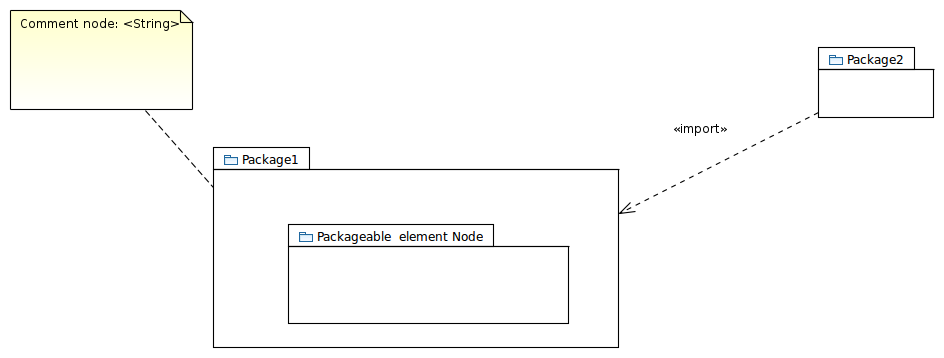
\includegraphics[width=\textwidth]{images/PackageDiagram.PNG}
  \caption{Package Diagram}
  \label{fig:package diagram}
\end{figure}


The following Package Diagram nodes and paths can be used for
modelling:
\begin{itemize}
\item Comment Note \sysmlicon{Comment.png}
\item Package Node \sysmlicon{Package.png}
\item Packageable Element Node
\item Import Path \sysmlicon{PackageImport.png}
\end{itemize}

The following items \emph{cannot} be used:
\begin{itemize}
\item Model Node
\item View Node
\item Viewpoint Node
\item Containenement Path
\item Dependency Path
\item Conform Path
\item Metamodel Node
\item Metaclass Node
\item Model Library Node
\item Stereotype Node
\item Profile Node
\item Generalization Path
\item Extension Path
\item Associatin Path
\item Reference Path
\item Profile Application Path
\end{itemize}

\subsection{Restrictions on Block Definition Diagram}



\begin{figure}[ht]
  \centering
  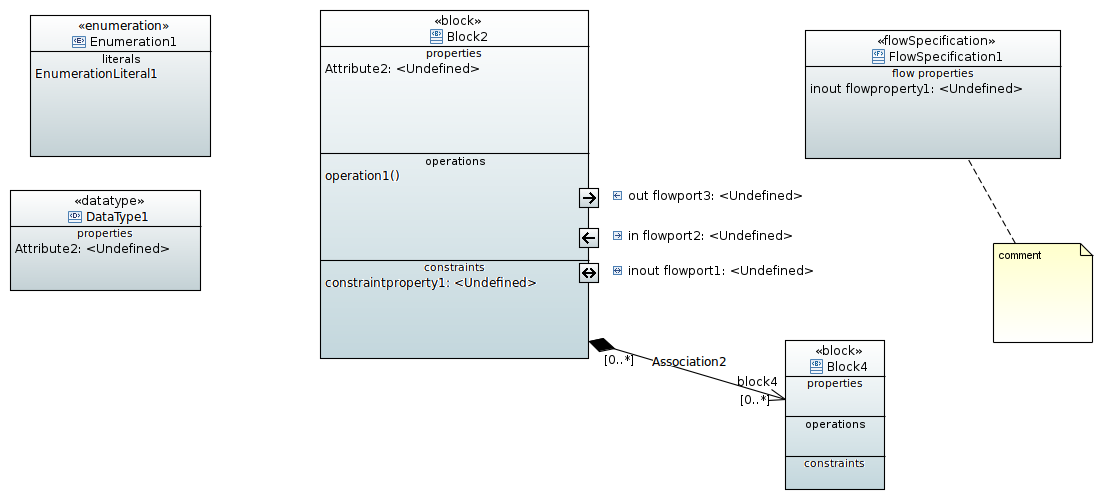
\includegraphics[width=\textwidth]{images/BDDDiagram.PNG}
  \caption{Block Description Diagram}
  \label{fig:Bdd}
\end{figure}



The following Block Definition Diagram nodes and paths can be used for
modelling:
\begin{itemize}
\item Block Node \sysmlicon{Block.png}
\item Enumeration Node \sysmlicon{Enumeration.png} and enumeration litteral
\item Block Node with ``datatype'' Stereotype \sysmlicon{DataType.png}
\item Composite Association Path \sysmlicon{Association_composite.png}
\item Flow Specification Node \sysmlicon{FlowSpecification.png} and Flow Properties
\item Primitive Type Node
\item Property Node
\item Constraint Node
\item Requirement Node
\end{itemize}

The following items \emph{cannot} be used:
\begin{itemize}
\item Quantity Kind and Unit Nodes
\item Value Type Node
\item Actor Node
\item Interface Block Node (SysML 1.3)
\item Interface Node
\item Signal Node
\item Interface Compartments for Block Node
\item Reference Association Path
\item Association Block Path and Node
\item Generalization Path
\item Full Port Node
\item Proxy Port Node
\item Proxy Port Node With Interfaces
\item Port Compartments for Block Node
\item Nonatomic Flow Port Node
\item Block Node with Constraint Compartment
\item Constraint Block Node
\item Activity Node
\item Activity Composition Path
\item Object Node Composition Path
\item Instance Specification Node
\item Association Instance Specification (Link) Path
\end{itemize}

\subsection{Restrictions on Internal Block Diagram}



\begin{figure}[ht]
  \centering
  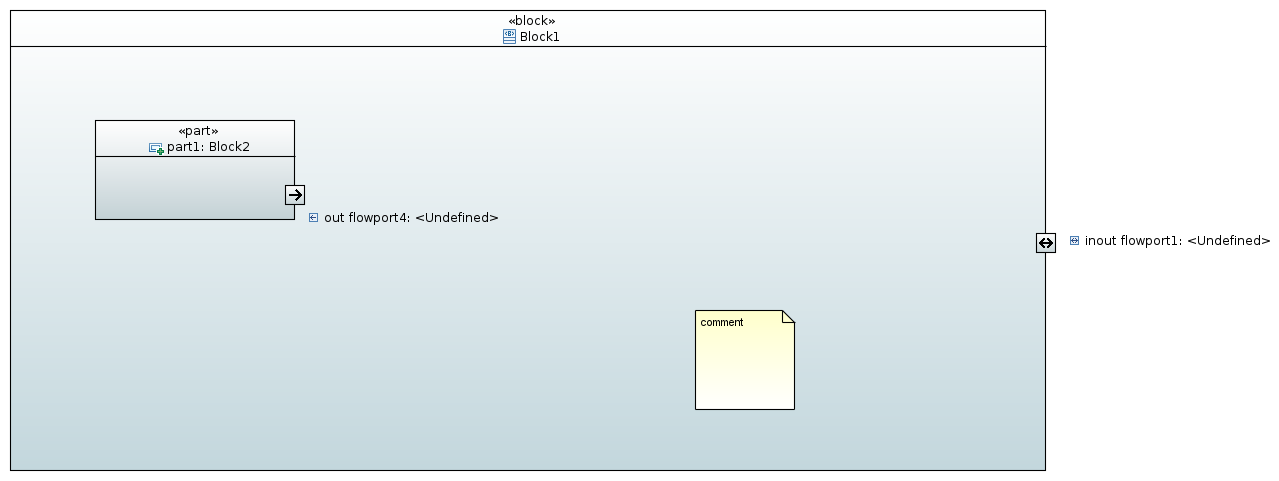
\includegraphics[width=\textwidth]{images/IBDDiagram.PNG}
  \caption{Internal Block Diagram}
  \label{fig:ibd}
\end{figure}


The following Internal Block Diagram nodes and paths can be used for
modelling:
\begin{itemize}
\item Part Node \sysmlicon{Property.png}~\textsf{Part}
\item Connector Path \sysmlicon{Connector.png}
\item Atomic Flow Port Node \sysmlicon{FlowPort.png}
  \sysmlicon{FlowPort_INOUT.png} \sysmlicon{FlowPort_IN.png}
  \sysmlicon{FlowPort_OUT.png}
\end{itemize}

The following items \emph{cannot} be used:
\begin{itemize}
\item Actor Part Node
\item Reference Node
\item Participant Property Node
\item Value Property Node
\item Connector Property Path and Node
\item Item Flow Node
\end{itemize}

\subsection{Restrictions on Sequence Diagram}



\begin{figure}[ht]
  \centering
  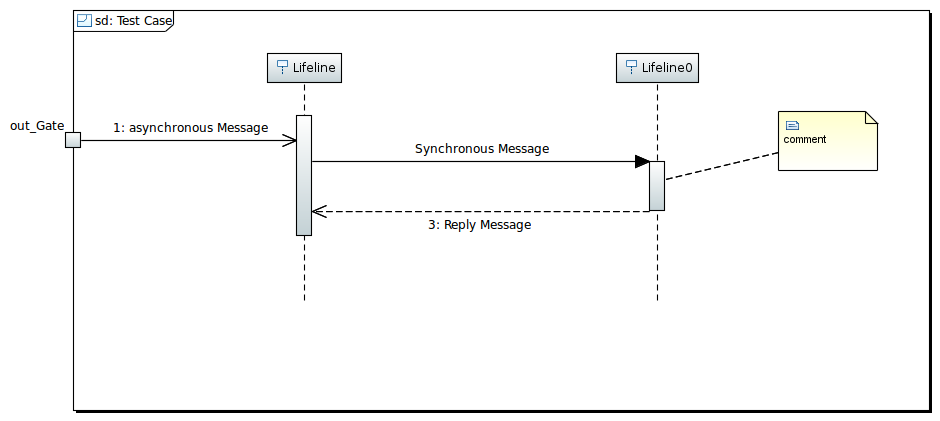
\includegraphics[width=\textwidth]{images/SequenceDiagram.PNG}
  \caption{Sequence Diagram}
  \label{fig:sd}
\end{figure}


The following Sequence Diagram nodes and paths can be used for
modelling:
\begin{itemize}
\item Lifeline Node \sysmlicon{Lifeline.png}
\item Synchronous Message \sysmlicon{Message_synchCall.png}
\item Asynchronous Message \sysmlicon{Message_asynchCall.png}
\item Reply Message \sysmlicon{Message_reply.png}
\end{itemize}

The following items \emph{cannot} be used:
\begin{itemize}
\item Single-compartment Fragment Node
\item Multi-compartment Fragment Node
\item Filtering Fragment Node
\item State Invariant Symbol
\item Interaction Use Node
\item Lost Message Path
\item Found Message Path
\item Activation Node
\item Create Message Path
\item Destroy Event Node
\item Coregion Symbol
\item Duration Observation Symbol
\item Duration Constraint Symbol
\item Time Observation Symbol
\item Time Constraint Symbol
\end{itemize}

\subsection{Restrictions on State Machine Diagram}



\begin{figure}[ht]
  \centering
  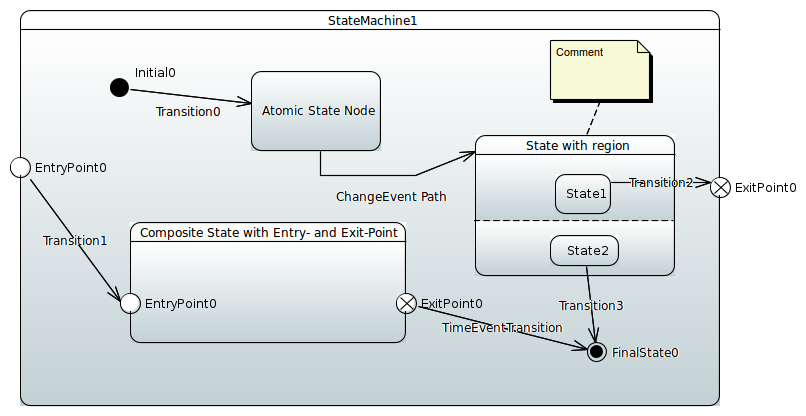
\includegraphics[width=\textwidth]{images/StateMachineDiagram.PNG}
  \caption{State Machine Diagram}
  \label{fig:sm diagram}
\end{figure}


The following State Machine Diagram nodes and paths can be used for
modelling:
\begin{itemize}
\item State Machine with Entry- and Exit-Point Pseudostate Nodes
\item Atomic State Node
\item Composite State with Entry- and Exit-Point Pseudostate Nodes
\item Composite State Node with Multiple Region
\item Initial Pseudostate Node
\item Final State Node
\item Time Event Transition Path
\item Change Event Transition Path
\item Constraint Node (for transition guard)
\item Constraint Path between state and constraint
\item Constraint Path between transition and constraint
\item Requirement Node (to link some diagram parts to a requirement)
\item Realize Path between state and requirement
\item Realize Path between constraint and requirement
\end{itemize}

Simple and composite states may contain internal activities
compartments:
\begin{itemize}
\item Entry actions may contain simple C-Assignments, timer resets or
  operation calls;
\item Exit actions may contain simple C-Assignments, timer resets or
  operation calls;
\item Do actions may contain simple C-Assignments, timer resets or
  operation calls.
\end{itemize}

The following items \emph{cannot} be used:
\begin{itemize}
\item Sub-State Machine Node with Connection Points
\item Terminate Pseudostate Node
\item Choice Pseudostate Node
\item Junction Pseudostate Node
\item Trigger Node
\item Action Node
\item Send Signal Node
\item Join Pseudostate Node
\item Frok Pseudostate Node
\item History Pseudostate Node
\item Signal Event Transition Path
\item Call Event Transition Path
\end{itemize}

\subsection{Restrictions on Requirement Diagram}

\begin{figure}[ht]
  \centering
  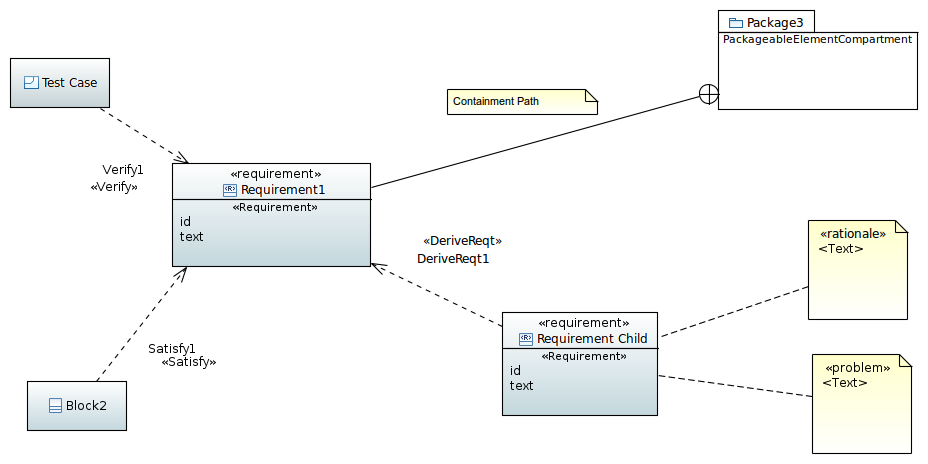
\includegraphics[width=\textwidth]{images/RequirementDiagram.PNG}
  \caption{Requirement Diagram}
  \label{fig:req diagram}
\end{figure}


The following Requirement Diagram nodes and paths can be used for
modelling:
\begin{itemize}
\item Requirement Node \sysmlicon{Requirement.png}
\item Package Node
\item Containment Path
\item Derivation Path \sysmlicon{DeriveReqt.png}
\item Satisfaction Path \sysmlicon{Satisfy.png}
\item Verification Path \sysmlicon{Verify.png}
\item Rationale Callout \sysmlicon{Rationale.png}
\item Problem Callout \sysmlicon{Problem.png}
\end{itemize}

The following items \emph{cannot} be used:
\begin{itemize}
\item Requirement Related-Type Node
\item Trace Compartment
\item Test Case Node
\item Refinement Path
\item Trace Path
\item Copy Path
\item Trace Callout
\item Derivation Callout
\item Verification Callout
\item Statisfaction Callout
\item Refinement Callout
\item Master Requirement Callout
\end{itemize}



\subsection{Model patterns}

For \emph{Modelling} activity, the modeler shall only use:
\begin{itemize}
\item \emph{Package Diagram}
\item \emph{Block Definition Diagram} (BDD)
\item \emph{Internal Block Diagram} (IBD)
\item \emph{State Machine Diagram}
\item \emph{Requirement Diagram}
\end{itemize}

For \emph{V\&V} activities, one shall only use:
\begin{itemize}
\item \emph{Package Diagram}
\item \emph{Block Definition Diagram} (BDD)
\item \emph{Internal Block Diagram} (IBD)
\item \emph{Sequence Diagram}
\item \emph{Requirement Diagram}
\end{itemize}

The following guidelines should be followed:
\begin{itemize}
\item Each block must either have an associated state machine diagram
  (with the same name).
\item Guard conditions contain Boolean conditions over variables and
  timer;
\item Actions are sequences of C assignments, timer resets or
  operation calls;
\item Initial state of a State Machine has only one out transition
  without guard condition or action.
\end{itemize}

\begin{comment}
FIXME: Example of patterns to use.

\end{comment}


% LocalWords:  SysML



\section{Approaches for low level design}

\begin{comment}
to  complete later: SCADE ? OS approaches ?
\end{comment}

%%%%%%%%%%%%%%%%%%%%%%%%%%%

%% Bibliography
\nocite{*}
\bibliographystyle{unsrt}
\bibliography{erdc}



% \begin{thebibliography}{9}

% \bibitem{lamport94}
  % Leslie Lamport,
  % \emph{\LaTeX: A Document Preparation System}.
  % Addison Wesley, Massachusetts,
  % 2nd Edition,
  % 1994.

% \end{thebibliography}

%===================================================
%Do NOT change anything below this line

\end{document}
